\documentclass[letterpaper,twocolumn,10pt]{article} 
\usepackage{usenix-2020-09}
\usepackage{graphicx}

% Proposal due date
\date{31st of October, 2022}

% Project Title
\title{%
  {\Large \bf An Interactive Visualizer for Equality Solvers using E-Graphs}\\%
  {\large Princeton University COS 516 Course Project (Fall '22)}%
}

%for single author (just remove % characters)
\author{ {\rm Ryan Torok}\\ Princeton University \and {\rm Leon Sch\"urmann}\\ Princeton University
% copy the following lines to add more authors \and {\rm Name}\\
%Name Institution
} % end author
\begin{document}

\maketitle

\section{Introduction}

The \textit{Theory of Equality} (TOE) is a theory in first-order logic which axiomatizes that the equality operator (=) behaves reasonably\cite{bm}. A well-known algorithm for finding all equivalence classes of a given formula, which constitutes a theory solver for TOE, is to list out all terms that appear in the formula, then iterate through pairs of terms, adding terms to equivalence classes using a union-find data structure by repeatedly applying the rule $a = b \rightarrow f(a) = f(b)$, where $a$ and $b$ are terms, and $f$ is a function symbol. In the worst case, running this procedure until no more matches are possible requires quadratic time. While this is still a polynomial-time algorithm, it is rather naive in its method to choose new pairs and it is definitely possible to do better.

E-graphs \cite{egraphs} improve the time complexity of this procedure by representing the terms of a formula as a directed acyclic graph (DAG), such that each constant symbol or function symbol is given a single node, and the composition of terms is represented by the edges. For example, Figure \ref{fig:egraph} represents an e-graph for the formula $(a * 2) / 2$. The structure of these graphs make it possible to efficiently find all equality classes without requiring the linear pass over all terms, and also make it possible to support an arbitrary set of additional rewrite rules. \texttt{egg} is a popular Rust library that implements e-graphs, and has seen frequent use in implementations of automated verification programs, largely due to its flexibility \cite{egg}.

\begin{figure}[t]
    \centering
    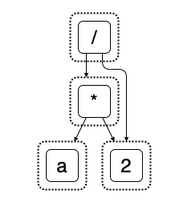
\includegraphics[width=.5\columnwidth]{egraph.png}
    \caption{E-graph representing the formula $(a * 2) / 2$}
    \label{fig:egraph}
\end{figure}

\begin{figure*}[t]
    \centering
    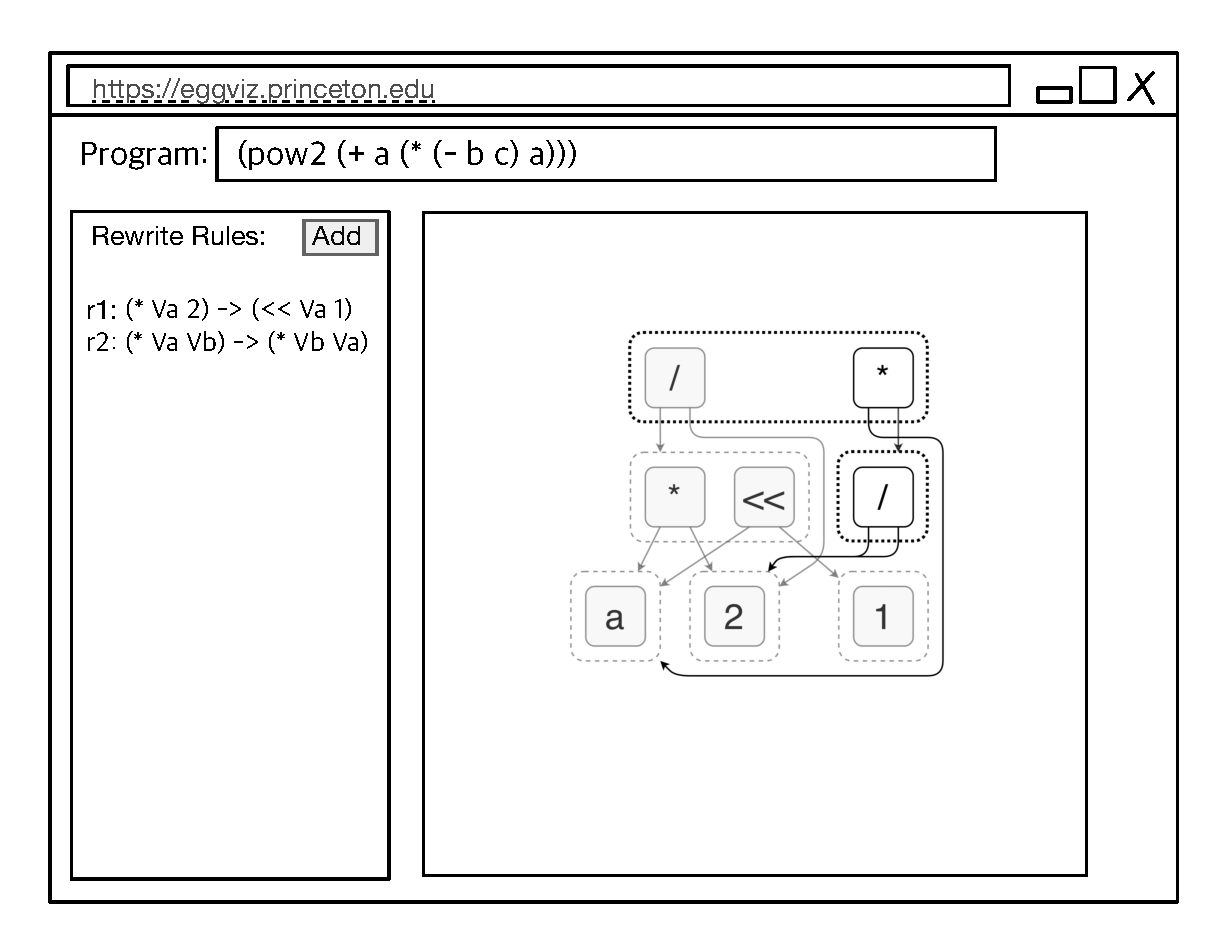
\includegraphics[width=.7\linewidth]{eggviz-ui.pdf}
    \caption{Illustration of our proposed web interface.}
    \label{fig:ui}
\end{figure*}

Unfortunately, the precise mechanisms employed both within the congruence closure algorithm, as well as the extended e-graph data structures, can be unintuitive for novice users. We presume that an interactive visualization can help demonstrate the basic concepts behind reasoning about equality under a given set of rewrite rules. In this project, we aim to create a web-based visualization tool that allows the user to interactively explore the equivalence-matching procedure and program optimization techniques in a step-by-step manner.

\section{Interface Design}


Figure \ref{fig:ui} shows a high-level layout of our proposed interface. Our web application will consist of an expression field, a left pane containing the set of user-defined rewrite rules, and a main view containing the e-graph. For the graph visualization, we plan to use the \texttt{vis} graph visualization library that was also used in the CDCL solver web application. The displayed graph will also indicate the found equivalence classes using either a dotted-line box (as in the \texttt{egg} paper), or using color coordination. As the user steps through the reduction, the visualization will indicate which equality classes are at each step and the responsible rewrite rule. We may also choose to support "tentative changes", where the user can hover over one of the classes in a possible merge and observe the effect without committing it.

The expression field will accept a program using prefix notation in a LISP-like syntax. For example, the program $\texttt{pow2(a + (b * c))}$ would be written as \texttt{(pow2 (+ a (* b c)))}. Requiring the user to enter programs in this format makes them simple to parse and has the particular advantage that the arity of each function symbol is fully deterministic and does not need to be manually specified by the user. The rewrite rules box will accept the same syntax, \mbox{as well as the \texttt{->} operator to represent "replaces"}.

\section{Implementation Strategy}

The system shall be implemented as a standalone web-application capable of running in modern Web browsers with WebAssembly support. It does not require any backend program and executes as a self-contained program in the user's web-browser.

In accordance with the requirements posed by the interface design section, the project shall implement a basic user interface in HTML5, CSS and JavaScript, possibly using preexisting user-interface and frontend application frameworks. This user interface incorporates a library for visualizing (intermediate) e-graphs maintained by the underlying application logic.

To actually represent the e-graph structure, as well as to perform any of the supported transformations and other operations (such as a step-by-step saturation of the e-graph), the system employs the \texttt{egg} library written in Rust. This library is extended with the necessary logic to interoperate with the frontend written in JavaScript, and embedded into the system  by means of compiling it to a WebAssembly library.

In order to integrate with our step-by-step visualization, we plan to transform \texttt{egg}'s equality saturation algorithm to allow our application read the intermediate state after each iteration of its loop, which we can use to produce a visualization of the application of rewrite rules.

\section{Possible Extensions}

It may be feasible to extend the application to not only operate on \texttt{egg}'s chosen order of rewrite rule applications, but to instead allow the user to guide applications of individual rewrite rules between terms of equivalence classes.

\section{Project Schedule}

We plan to build the proposed application by following roughly these steps:
\begin{enumerate}
    \item Build the basic project scaffold with a rudimentary frontend and an \texttt{egg} dummy application (\textit{1 week}).
    \item Implement parsing of the entered program (automatically deducing function \& constant symbols and creating appropriate Rust types to integrate with \texttt{egg}), as well as parsing of the rewrite rules (\textit{1 week}).
    \item Change \texttt{egg}'s implemented equivalence saturation algorithm to provide a step-by-step interface and return additional context for integration of our visualization (\textit{1-2 weeks}).
    \item Implement a JavaScript-based visualization for (intermediate) e-graphs. This likely includes a routine to walk two e-graphs and create a \textit{diff} to update a pre-existing rendered e-graph (\textit{1-2 weeks}).
    \item Finish and debug the implementation; write the project report (\textit{2 weeks}).
\end{enumerate}

\bibliographystyle{plain}
\bibliography{proposal}

\end{document}
